\chapter{Sistemi idrostatici}
Definiamo informalmente un sistema idrostatico come un sistema termodinamico determinato da pressione, volume e temperatura.


\begin{definition}[Principali processi quasistatici per sistemi idrostatici]
Un processo si dice
\begin{itemize}
\item \textbf{isotermo} se $T$ resta costante,
\item \textbf{isobaro} se $p$ resta costante,
\item \textbf{isocore} se $V$ resta costante o
\item \textbf{adiabatico} se non avviene scambio di calore.
\end{itemize}
\end{definition}

\section{Differenziale di volume}
\begin{definition}[Coefficiente di espansione volumetrica]
Definiamo il \textbf{coefficiente di espansione volumetrica} come
\[\al=\frac1V\ppb TVp=-\frac mV\frac1{\rho^2}\ppb T\rho p=-\frac1\rho\ppb T\rho p.\]
L'unit\`a di misura \`e $[\al]=\mathrm{K}\ii$.
\end{definition}


\begin{definition}[Compressibilit\`a isoterma]
Definiamo la \textbf{compressibilit\`a isoterma} come
\[\beta_T=-\frac1V\ppb pVT.\]
L'unit\`a di misura \`e $[\beta_T]=\mathrm{Pa}\ii$.\\
L'inversa $k_T=1/\beta_T$ \`e detta \textbf{modulo di compressibilit\`a isoterma}.
\end{definition}

\noindent Riportiamo alcuni valori di $\al$ e $\beta_T$ per dare una intuizione sui valori tipici\footnote{il Sitall \`e materiale fatto apposta per avere coefficiente di espansione volumetrica piccolo}
\begin{center}
\begin{tabular}[ht]{|c|c|c|}
\hline 
Materiale&$\al\ [\mathrm{K}\ii]$&$\beta_T\ [\mathrm{Pa}\ii]$\\\hline
Acqua&$0.2\cdot 10^{-3}$&$4.6\cdot 10^{-10}$\\
Diamante&$3\cdot 10^{-6}$&?\\
Sitall&$\leq 10^{-7}$&?\\
Sabbia&?&$\sim10^{-8}$\\
Mercurio&$1.8\cdot 10^{-4}$&$4\cdot10^{-11}$\\
Rame&?&$7.2\cdot10^{-12}$\\
\hline
\end{tabular}
\end{center}


\begin{remark}
Non \`e necessario battezzare $\displaystyle\ppb TpV$ in quanto per la propriet\`a ciclica (\ref{ProprietaDerivateParziali})
\[\ppb TpV=-\ppb VpT\ppb TVp=\frac\al{\beta_T}.\]
\end{remark}

\begin{remark}[Relazione differenziale tra $\al$ e $\beta_T$]
Per il teorema di Schwarz si ha che
\[\pp{p\del T}{^2V}=\ppb p\al T=-\ppb T{\beta_T}p.\]
\end{remark}

\begin{remark}[Differenziale del volume]
Dalle definizioni date segue che
\[dV=\al VdT-\beta_T Vdp.\]
\end{remark}

\begin{proposition}[Differenziale della pressione]\label{DifferenzialePressione}
Si ha che
\[dp=\frac\al{\beta_T}dT-\frac1{\beta_T V}dV.\]
\end{proposition}
\begin{proof}
Osserviamo che
\[\ppb TpV\pasgnl={(\ref{ProprietaDerivateParziali})}-\ppb VpT \ppb TVp=\frac \al{\beta_T},\]
dunque ricaviamo
\[dp=\ppb TpVdT+\ppb VpT=\frac\al{\beta_T}dT-\frac1{\beta_T V}dV.\]
\end{proof}
\begin{corollary}
In una trasformazione isocora $\Delta p=\frac\al{\beta_T}\Delta T$.
\end{corollary}

\begin{remark}[Differenziale logaritmico nel volume]\label{DifferenzialeLogaritmicoNelVolume}
Spesso torner\`a comodo ricordare il seguente sviluppo differenziale
\[d\log V=\frac1VdV=\al dT-\beta_T dp\]
\end{remark}
\begin{proof}
Segue calcolando:
\[\frac1VdV=\frac1V\pa{\ppb TVp dT+\ppb pVTdp}=\al dT-\beta_T dp\]
\end{proof}

\section{Lavoro per sistema idrostatico}
Immaginiamo di comprimere un sistema idrostatico come in figura 

\begin{figure}[!htb]
	\centering
	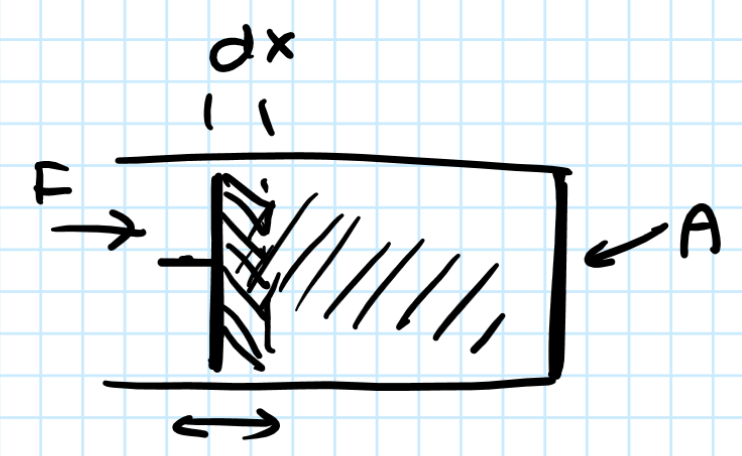
\includegraphics[width=4cm]{images/Lavoro_In_Idrostatico.png}
\end{figure}


\noindent
Se spingiamo molto lentamente possiamo con buona approssimazione supporre che il processo sia quasistatico, dunque $F=pA$. Segue che
\[\boxed{\delta W=Fdx=pAdx}\]
Se il sistema in questione \`e un gas ideale allora
\[\delta W=p(-dV)=-pdV\]
Il lavoro totale per passare da uno stato $A$ ad uno stato $B$ diventa
\[W=-\int_{A}^{B} p(V,T)dV,\]
ma $p$ come cambia al variare di $V$? Dipende dal tipo di processo.

\begin{figure}[!htb]
	\centering
	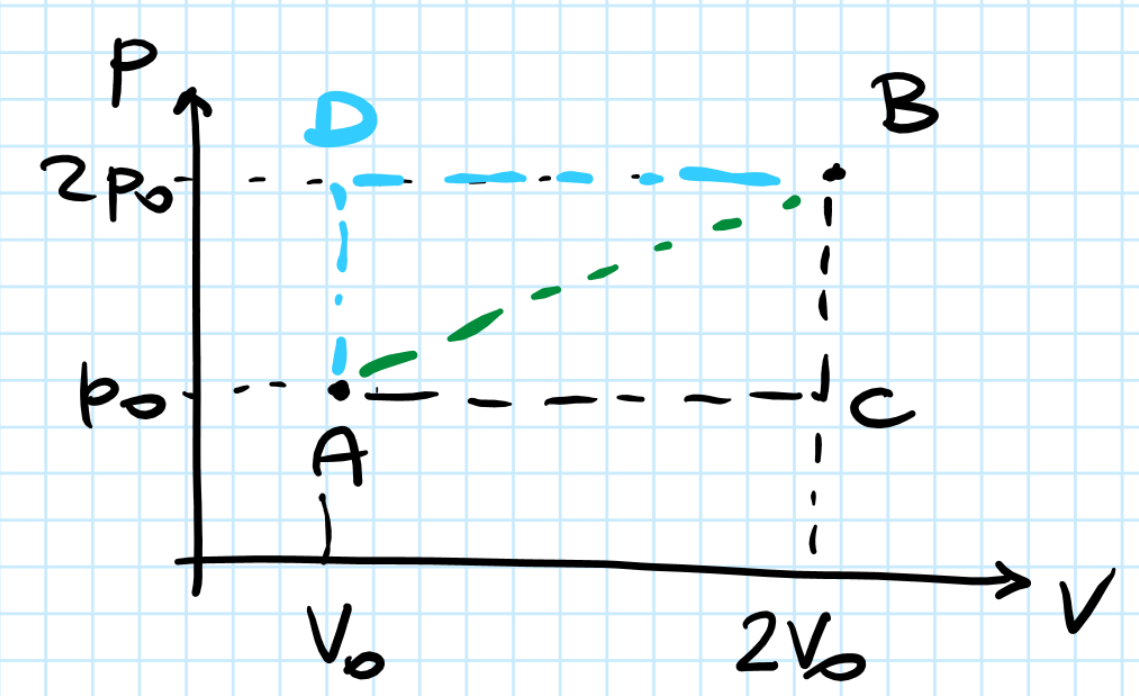
\includegraphics[width=5cm]{images/Lavoro_non_e_funzione_di_stato.png}
\end{figure}

\noindent
Questo mostra in particolare che il lavoro non \`e una funzione di stato.

\section{Capacit\`a termica}
\begin{definition}[Capacit\`a termica]
Definiamo la \textbf{capacit\`a termica} come\footnote{Nota che NON \`e una derivata in quanto $Q$ non \`e una funzione di stato, quindi in particolare non \`e una funzione di $T$}
\[C=\lim_{\delta T\to 0}\frac{\delta Q}{\delta T}.\]
L'unit\`a di misura \`e $[C]=\mathrm{J}/\mathrm{K}$.\\
La \textbf{capacit\`a termica molare} \`e data da $c=C/n$.\\
Il \textbf{calore specifico} \`e dato da $C/m$.
\end{definition}

\begin{definition}[Caloria]
Una \textbf{caloria} \`e la quantit\`a di calore necessaria per far variare la temperatura di un grammo di acqua da $14.5^\circ\mathrm{C}$ a $15.5^\circ\mathrm{C}$.\\
In Joule si ha che
\[\boxed{1\ \mathrm{cal}=4.186\ \mathrm{J}}\]
\end{definition}
\begin{remark}
Il calore specifico dell'acqua per temperature ragionevoli \`e
\[c_{\text{acqua}}=4.186\frac{\mathrm{J}}{^\circ\mathrm{C}\ \mathrm{g}}=4186\frac{\mathrm{J}}{\mathrm{K}\ \mathrm{kg}}\]
\end{remark}

\begin{definition}[Termometro e Termostato]
Un \textbf{termostato} \`e un oggetto ideale con capacit\`a termica infinita\footnote{intuitivamente \`e un sistema grande a sufficienza in modo che anche se viene aggiunto calore, la temperatura non cambia.}.\\ 
Un \textbf{termometro} \`e un oggetto ideale con capacit\`a termica nulla\footnote{intuitivamente \`e un sistema piccolo a sufficienza in modo da poter trascurare gli scambi di calore.}.
\end{definition}

\begin{remark}
Possiamo scrivere la capacit\`a termica in termini di $U,\ V,\ p$ e $T$ come segue:
\[C=\frac{\delta Q}{\delta T}=\ppb TUV+\pa{\ppb VUT+p}\dd TV\]
\end{remark}
\begin{proof}
Sviluppando $dU$ troviamo
\[dU=\ppb TUVdT+\ppb VUTdV,\]
da cui
\[\delta Q=dU+pdV=\ppb TUVdT+\pa{\ppb VUT+p}dV.\]
Ora possiamo ``dividere" per $dT$ e trovare la tesi.
\end{proof}

\begin{definition}[Capacit\`a termica a volume/pressione costante]
Definiamo la \textbf{capacit\`a termica a volume} (risp. \textbf{pressione}) \textbf{costante} come le due seguenti quantit\`a
\begin{align*}
C_V=&\rbar{\frac{\delta Q}{\delta T}}_V=\ppb TUV\\
C_p=&\rbar{\frac{\delta Q}{\delta T}}_p=\ppb TUV +\pa{\ppb VUT+p}\ppb TVp=\ppb TUV +\pa{\ppb VUT+p}V\al
\end{align*}
\end{definition}

\begin{remark}[Disuguaglianza tra capacit\`a termiche]\label{DisguguaglianzaCapacitaTermiche}
Vale sempre $C_p>C_V$.
\end{remark}

\begin{remark}\label{DerivataEnergiaInternaRispettoAlVolume}
In un gas generale
\[\boxed{\ppb VUT=\frac{C_p-C_V}{V\al}-p}\]
\end{remark}

\subsection{Processi politropici}
Possiamo generalizzare i quattro tipi di processi principali come segue:
\begin{definition}[Processo politropico]
Un processo \`e \textbf{politropico} se la capacit\`a termica \`e costante.
\end{definition}

\begin{proposition}[Curve per processi politropici]\label{CurveProcessiPolitropici}
Considerando un processo politropico relativo ad un gas ideale e definiamo
\[\delta=\frac{C_p-C}{C_V-C},\]
allora seguendo questo processo si ha che $pV^\delta=cost.$.
\end{proposition}
\begin{proof}
Poich\'e $\delta Q=CdT=C_VdT+pdV=C_pdT-Vdp$ ricaviamo che
\[-\frac V{C-C_p}dp=dT=\frac p{C-C_V}dV,\]
da cui
\[-\frac Vp\dd Vp=\frac{C_p-C}{C_V-C}=\delta.\]
Questa espressione restituisce una equazione differenziale
\[-\frac{dp}p=\delta\frac{dV}V,\]
la cui soluzioni hanno la forma voluta.
\end{proof}

\noindent
Possiamo interpretare processi isocori, isobari, isotermi e adiabatici come processi politropici:
\begin{center}
\begin{tabular}[ht]{|c||c|c|c|c|}
\hline
Processo & Isocoro & Isobaro & Isotermo & Adiabatico\\\hline&&&&\\
$\delta$ & $\infty$ & $0$ & $1$ & $\displaystyle\gamma=\frac{c_p}{c_V}$\\ &&&&\\\hline
\end{tabular}
\end{center}



\section{Potenziali termodinamici}
\subsection{Energia interna ed entropia}

\begin{remark}[Differenziali]
Osserviamo che
\[TdS=\rbar{\delta Q}_{rev}=dU-\rbar{\delta W}_{rev}=dU+pdV,\]
dunque
\[\boxed{dU=TdS-pdV}\]
\end{remark}
\begin{remark}
\underline{\textbf{NOTA BENE:}} Questo sembra un altro modo di scrivere il primo principio $dU=\delta Q+\delta W$, ma se il processo non \`e reversibile allora non \`e detto che $pdV=\delta W$.
\end{remark}

\begin{proposition}[Equazione di Helmholtz]\label{EquazioneHelmholtz}
Vale la seguente identit\`a
\[\boxed{\ppb VUT=T\ppb TpV-p}=T^2\ppb T{(p/T)}V\]
\end{proposition}
\begin{proof}
Sviluppiamo il differenziale dell'entropia
\[dS=\frac{dU}T+\frac{pdV}T=\frac1T\pa{\ppb TUVdT+\ppb VUTdV}+\frac pTdV.\]
Poich\'e $dS$ \`e un differenziale esatto, le derivate incrociate devono coincidere:
\begin{gather*}
\pp V{}\pa{\frac1T\ppb TUV}=\rbar{\pp T{}\pa{\frac1T\pa{\ppb VUT+p}}}_V\\
\cancel{\frac1T\pp{V\del T}{^2U}}=-\frac1{T^2}\pa{\ppb VUT+p}+\cancel{\frac1T\pp{V\del T}{^2U}}+\frac1T\ppb TpV\\
\ppb VUT=T\ppb TpV-p.
\end{gather*}
\end{proof}
\begin{remark}
Osserviamo che 
\[dU=\under{=C_V}{\ppb TUV}dT+\ppb VUTdV,\]
quindi la formula di Helmholtz misura ``quanto un gas non \`e ideale" (ricordiamo (\ref{DerivataEnergiaInternaRispettoAlVolume}))
\end{remark}
\begin{remark}
Se $dU=0$ allora
\[dT=-\frac{\ppb VUT}{\ppb TUV}dV=\ppb VTUdV\pasgnl={(\ref{EquazioneHelmholtz})}\frac1{C_V}\pa{p-T\ppb TpV}dV.\]
Questa identit\`a pu\`o essere interpretata come test per Gas ideali, basta capire se $T\ppb pTV$ coincide con $\frac{nRT}V$.
\end{remark}

\begin{remark}
Valgono le seguenti identit\`a
\[C_V=T\ppb TSV,\quad C_p=T\ppb TSp,\qquad \gamma=\frac{\ppb VpS}{\ppb Vpp}=\frac{\beta_T}{\beta_S}\]
\end{remark}
\begin{proof}
ESERCIZIO
\end{proof}





\subsection{Entalpia}



\begin{definition}[Entalpia]
L'\textbf{entalpia} in un gas \`e definita da\footnote{cio\`e l'energia interna sommata al ``lavoro necessario per portare il volume da $0$ a $V$ a pressione costante".}
\[H=U+pV.\]
\end{definition}

\begin{remark}
L'entalpia \`e ottenuta da $U$ come trasformazione di Legendre:\\
Consideriamo $U(S,V)$ e cambiamo la coordinata $V$ in $-p=\ppb VUS$, che possiamo fare ponendo $H(S,p)=U-(-pV)=U+pV$.
\end{remark}

\begin{remark}[Differenziale dell'entalpia]
Il differenziale di $H$ \`e dato da
\[dH=dU+pdV+Vdp=TdS+Vdp\pasgnl={se reversibile}\delta Q+Vdp\]
oppure da
\[dH=dU+p(\al VdT-\beta_T Vdp)+Vdp=dU+p\al VdT+V(1-\beta_Tp)dp.\]
\end{remark}
\begin{corollary}
Valgono le seguenti identit\`a
\[\ppb SHp=T,\quad \ppb pHS=V,\quad \ppb THp=C_p.\]
\end{corollary}
\begin{proof}
Le prime due seguono immediatamente da $dH=TdS+Vdp$, mentre l'ultima segue sviluppando la definizione di $C_p$:
\[C_p=\rbar{\frac{\delta Q}{\delta T}}_p=\ppb TUp+p\ppb TVp=\rbar{\pp T{}(U+pV)}_p=\ppb THp.\]
\end{proof}




\begin{definition}[Coefficiente di Joule-Thomson]
Definiamo il \textbf{coefficiente di Joule-Thomson} come
\[\mu_{JT}=\ppb pTH.\]
\end{definition}
\begin{fact}
Per ogni gas esiste una temperatura, detta \textbf{temperatura di inversione}, tale che sotto questa temperatura $\mu_{JT}>0$
\end{fact}




\subsection{Energia libera di Helmholtz e Gibbs}
\noindent
Diamo un nome alle rimanenti trasformazioni di Legendre di $U$:
\begin{definition}[Energia libera di Helmholtz]
Dall'energia interna cambiamo $S$ in $\ppb SUV=T$, definendo $F=U-TS$, detta \textbf{energia libera di Helmholtz}. Osserviamo che
\[dF=-SdT-pdV.\]
\end{definition}

\begin{remark}
L'energia libera di Helmholtz ci permette di ricavare il ``massimo lavoro estraibile tra due stati".
\end{remark}
\begin{proof}
Per il secondo principio $Q/T\leq \Delta S$, dunque
\[W=\Delta U-Q\geq \Delta U-T\Delta S=\Delta F,\]
cio\`e il lavoro che pu\`o fare il sistema ($-W$) \`e al massimo $-\Delta F$.
\end{proof}

\begin{remark}
Si ha che
\[\ppb TFV=-S,\quad \ppb VFT=-p.\]
\end{remark}

\begin{definition}[Energia libera di Gibbs]
Dall'entalpia cambiamo $S$ in $\ppb SHp=T$, definendo $G=H-TS=U+pdV-TS=F+pV$, detta \textbf{energia libera di Gibbs}. Osserviamo che
\[dG=-SdT-Vdp.\]
\end{definition}

\begin{remark}
Si ha che
\[\ppb pGT=V,\quad \ppb TGp=-S.\]
\end{remark}

\begin{proposition}[Secondo principio per energia libera di Gibbs]\label{GibbsDiminuiscePerPressioneETemperaturaCostanti}
Se $T$ e $p$ sono costanti l'energia libera di Gibbs tende a diminuire.
\end{proposition}
\begin{proof}
Per il secondo principio $TdS-\delta Q\geq 0$. Sviluppando $\delta Q$ troviamo
\[TdS-dU-pdV\geq0.\]
Se $p$ \`e costante allora $dH=dU+pdV$, quindi in tal caso
\[TdS-dH\geq 0\]
Se ora $T$ resta costante si ha che $dG=dH-TdS$, cio\`e
\[dG\leq 0.\]
Segue dunque che se $T$ e $p$ sono costanti, $G$ tende a diminuire.
\end{proof}


\begin{proposition}[Relazioni di Maxwell]\label{RelazioniMaxwell}
Valgono anche le equazioni
\[\ppb VTS=-\ppb SpV,\quad \ppb pTS=\ppb SVp,\quad \ppb VST=\ppb TpV,\quad \ppb pST=-\ppb TVp.\]
\end{proposition}
\begin{proof}
Derivano dall'eguagliare derivate seconde delle energie che abbiamo definito. In ordine le quattro equazioni sono uguali a
\[\pp[2]{V\del S}U,\quad \pp[2]{p\del S}H,\quad -\pp[2]{V\del T}F,\quad \pp[2]{p\del T}G.\]
\end{proof}

\begin{remark}[Jacobiano $p,V$ - $T,S$]
Possiamo derivare le relazioni di Maxwell anche constatando che
\[\pp{(p,V)}{(T,S)}=1.\]
\end{remark}
\begin{proof}
Mostriamo che l'identit\`a vale e poi ricaviamo le relazioni da essa.
\setlength{\leftmargini}{0cm}
\begin{itemize}
\item[$\boxed{dPdV=dTdS}$] Per il primo principio
\[dU=TdS-PdV\leadsto 0=d^2U=dTdS-dPdV,\]
segue dunque per unicit\`a della scrittura in base che lo Jacobiano in esame vale $1$.
\item[$\boxed{\text{Relazioni}}$] Ricaviamo la prima, le altre seguono in modo analogo
\[\ppb VTS=\pp{(V,S)}{(T,S)}=\pa{\pp{(p,V)}{(T,S)}}\ii\pp{(V,S)}{(T,S)}=\pp{(V,S)}{(p,V)}=-\pp{(S,V)}{(p,V)}=-\ppb SpV.\]
\end{itemize}
\setlength{\leftmargini}{0.5cm}
\end{proof}




\subsection{Riassunto}
Riassumiamo il comportamento di queste quantit\`a nella seguente tabella:
\begin{center}
\begin{tabular}{|c||c|c|c|}
\hline
Energia & Definizione &Differenziale & Rel. Maxwell\\\hline
Interna & $\Delta U=Q+W$ & $+TdS-p\ dV$ & $\ppb VTS=-\ppb SpV$\\
Entalpia & $H=U+pV$ & $+TdS+Vdp$ & $\ppb pTS=\ppb SVp$\\
Helmholtz & $F=U-TS$ & $-SdT-p\ dV$ & $\ppb VST=\ppb TpV$\\
Gibbs & $G=U+pV-TS$ & $-SdT+Vdp$ & $-\ppb pST=\ppb TVp$\\\hline
\end{tabular}
\end{center}
Mettendo a confronto energia interna ed entalpia troviamo ulteriori similitudini:
\begingroup
\renewcommand{\arraystretch}{1.5}
\begin{center}
\begin{tabular}{|c||c||c|}
\hline
Argomento & Energia interna & Entalpia\\\hline\hline
Espansione & libera di Joule & di Joule-Thompson\\\hline
Quanto non ideale?& $\mu_J=\ppb VTU$ & $\mu_{JT}=\ppb pTH$\\\hline
Differenziale reversibile &$dU=\delta Q-pdV$ & $dH =\delta Q+Vdp$\\\hline
C. di Esp. Termica&$C_V=\ppb TUV$ & $C_p=\ppb THp$\\\hline
Su isocora & $\Delta U=Q$ & $\Delta H=Q$\\\hline
Su adiabatica & $\Delta U=-\int pdV$ &  $\Delta H=\int Vdp$\\\hline
In gas ideale & $\Delta U=\int c_VdT$ & $\Delta H=\int c_pdT$\\\hline
\end{tabular}
\end{center}
\endgroup

\bigskip
\noindent
Per ricordare le varie derivate parziali pu\`o essere utile il \textbf{diagramma di Konis-Born}
% https://q.uiver.app/#q=WzAsNCxbMCwwLCJUIl0sWzEsMCwiViJdLFswLDEsIlAiXSxbMSwxLCJTIl0sWzIsMywiSCIsMix7InN0eWxlIjp7ImhlYWQiOnsibmFtZSI6Im5vbmUifX19XSxbMCwxLCJGIiwwLHsic3R5bGUiOnsiaGVhZCI6eyJuYW1lIjoibm9uZSJ9fX1dLFsxLDMsIlUiLDAseyJzdHlsZSI6eyJoZWFkIjp7Im5hbWUiOiJub25lIn19fV0sWzAsMiwiRyIsMix7InN0eWxlIjp7ImhlYWQiOnsibmFtZSI6Im5vbmUifX19XSxbMiwxLCIiLDMseyJsYWJlbF9wb3NpdGlvbiI6NjAsInN0eWxlIjp7InRhaWwiOnsibmFtZSI6Im1vbm8ifX19XSxbMywwLCIiLDEseyJzdHlsZSI6eyJ0YWlsIjp7Im5hbWUiOiJtb25vIn19fV1d
\[\begin{tikzcd}
	T & V \\
	p & S
	\arrow["H"', no head, from=2-1, to=2-2]
	\arrow["F", no head, from=1-1, to=1-2]
	\arrow["U", no head, from=1-2, to=2-2]
	\arrow["G"', no head, from=1-1, to=2-1]
	\arrow[tail, from=2-1, to=1-2]
	\arrow[tail, from=2-2, to=1-1]
\end{tikzcd}\]
I due vertici di uno stesso lato contengono le variabili che appaiono nei differenziali mentre le diagonali indicano il valore della derivata dell'energia di un dato lato per la variabile del vertice. Il verso delle diagonali indica il segno di queste derivata, quindi per esempio per il lato destro ricaviamo
\[\ppb SUV=T,\quad \ppb VUS=-p.\]
Le due coppie di lati opposti corrispondono ognuna a due relazioni di Maxwell. Per capire i segni basta considerare i due triangoli che si formano scegliendo uno degli altri lati e completando con le due diagonali, per esempio la relazione
\[\ppb VTS=-\ppb SpV\]
si pu\`o leggere associando al membro di sinistra il triangolo $TVS$ e a quello di destra il triangolo $pSV$.

\section{Sistemi aperti di gas}
Per sistemi di gas aperto
\[\Delta U=Q+W+\Delta U_{materia},\]
o in forma differenziale
\[dU=TdS-pdV+\mu dn\]
dove $\mu$ \`e il \textbf{potenziale chimico}.
\begin{remark}
Valgono le identit\`a differenziali
\[\ppb SU{V,n}=T,\qquad \ppb VU{S,n}=-p,\qquad \ppb nU{S,V}=\mu.\]
\end{remark}
